\documentclass{article}

\usepackage{lipsum}
\usepackage[margin=1in,includefoot]{geometry}
\usepackage{graphicx} %For inserting images
\graphicspath{}

\begin{document}

\title{Simplified Kinematics of a Robotic Arm}
\author{}
\date{}
\maketitle

\section*{Derivation}
There are three arm linkages on the robotic arm. Assuming the outer most arm linkage is vertical and the two inner arms are of equal length $l$, it is fairly straightforward to calculate the angles between arm linkages. For the motors being used (NEMA 17 Stepper Motors), 200 steps corresponds to one full rotation. By calculating the desired angles for the motors, it is simple enough to calculate the number of steps that must be sent to them. 
\begin{center} 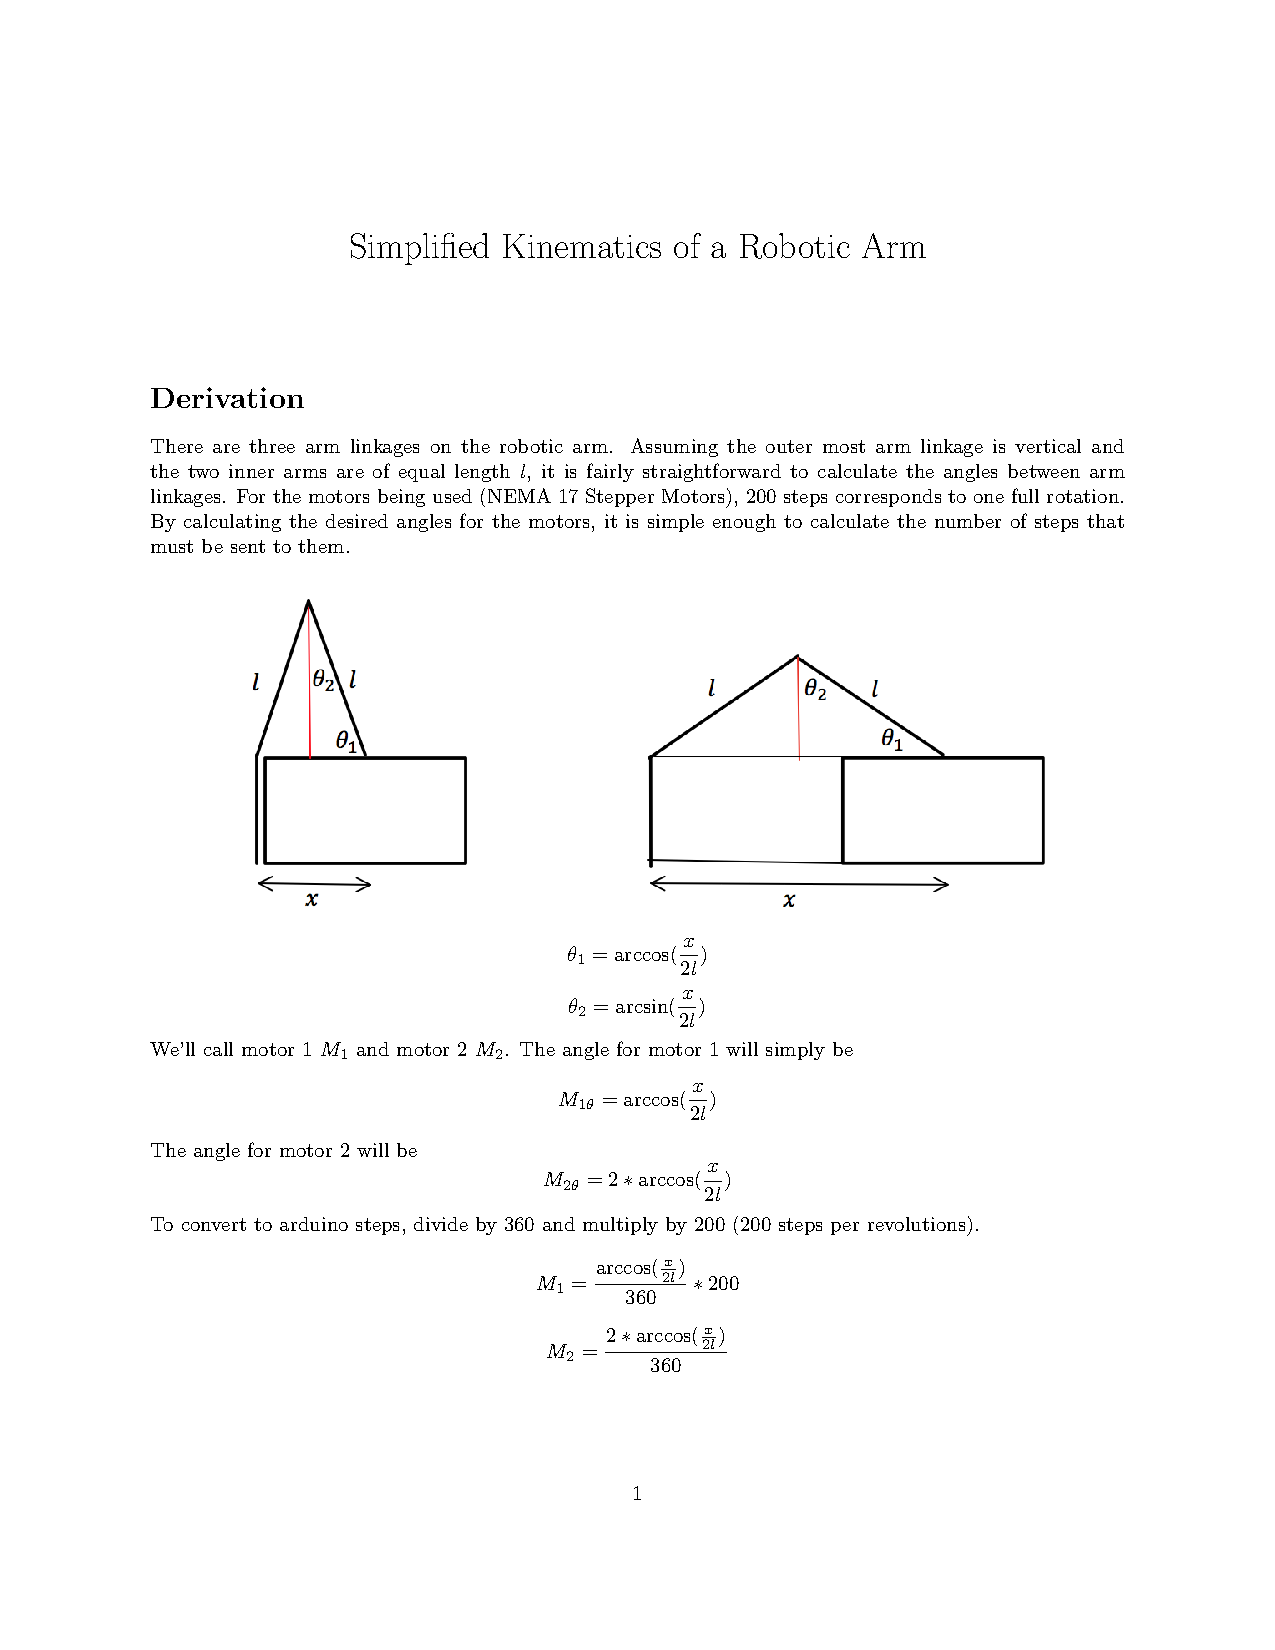
\includegraphics[scale=.8]{kinematics}  \end{center}
$$ \theta_1 = \arccos(\frac{x}{2l}) $$
$$ \theta_2 = \arcsin(\frac{x}{2l}) $$
We'll call motor 1 $M_1$ and motor 2 $M_2$. The angle for motor 1 will simply be 
$$ M_{1\theta} = \arccos(\frac{x}{2l}) $$
The angle for motor 2 will be 
$$ M_{2\theta} = 2*\arccos(\frac{x}{2l}) $$
To convert to arduino steps, divide by 360 and multiply by 200 (200 steps per revolutions). 
$$ M_{1} = \frac{\arccos(\frac{x}{2l})}{360}*200 $$
$$ M_{2} = \frac{2*\arccos(\frac{x}{2l})}{360} $$


\end{document}

